%% Figure from MATH 556 notes, section 46 (Lecture 20). ADDED (not from lecture).
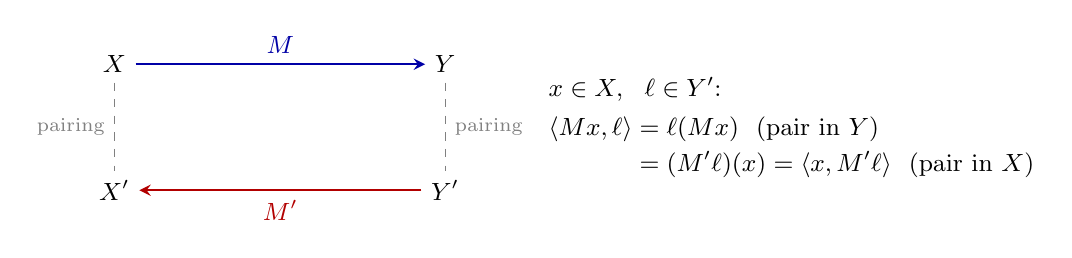
\begin{tikzpicture}[>=stealth, every node/.style={font=\small}]
  \node (X) at (0,1.6) {$X$};
  \node (Y) at (4.2,1.6) {$Y$};
  \node (Xp) at (0,0) {$X'$};
  \node (Yp) at (4.2,0) {$Y'$};
  \draw[->, thick, blue!65!black] (X) -- node[above] {$M$} (Y);
  \draw[->, thick, red!70!black] (Yp) -- node[below] {$M'$} (Xp);
  \draw[dashed, gray] (X) -- node[left, font=\scriptsize] {pairing} (Xp);
  \draw[dashed, gray] (Y) -- node[right, font=\scriptsize] {pairing} (Yp);
  \node[align=left, font=\small] at (8.6,0.8) {$x \in X,\ \ \ell \in Y'$:\\[3pt] $\langle Mx, \ell \rangle = \ell(Mx)$ \ (pair in $Y$)\\[2pt] $\phantom{\langle Mx, \ell \rangle} = (M'\ell)(x) = \langle x, M'\ell \rangle$ \ (pair in $X$)};
\end{tikzpicture}
